\documentclass[11pt]{article}
\usepackage{icmlko}
\begin{document}

\title{두 번째 짝도 오른다 --- 안 본 도메인 둘에서 같은 기계}
\author{월드모델 실험실}
\date{노트 418 · 2026년 8월 2일}
\maketitle

\begin{abstract}
노트 417이 \texttt{grp} 로 KR 만화 전이를 $-0.1261 \to +0.2128$ 로 올리면서
두 가지를 남겼다 --- \emph{$+0.2128$ 의 오차를 모른다}, \emph{비게임 앱을
grp 로 다시 재야 한다}. 둘 다 닫는다.

\textbf{오차}: 씨앗 여덟이 $+0.2089 \sim +0.2245$(SD $0.0054$)라 씨앗 잡음이
아니고, 유보 322행 되뽑기 800회가 \textbf{95\% 구간
$[+0.0993, +0.3115]$} 에 \textbf{0 보다 큰 되뽑기 $1.000$} 이다.
\textbf{크기는 불확실하고 부호는 확실하다.}

\textbf{두 번째 짝}: 비게임 앱은 학습에 한 번도 안 들어간 열두 번째
도메인이다(노트 397).

\begin{center}
\begin{tabular}{lrrr}
\hline
안 본 도메인 & grp 없음 & \textbf{grp 있음} & 차 \\
\hline
KR 만화 (유보 322) & $-0.0822$ & $\mathbf{+0.2128}$ & $+0.2950$ \\
비게임 앱 전부 (1{,}600) & $+0.0421$ & $\mathbf{+0.1474}$ & $+0.1053$ \\
비게임 앱 2025$+$ (189) & $+0.2304$ & $\mathbf{+0.2602}$ & $+0.0298$ \\
\hline
\end{tabular}
\end{center}

\textbf{둘 다 오른다.} 씨앗 SD 는 $0.005 \sim 0.007$ 로 작다. 노트 417의
기계가 \textbf{한 도메인의 우연이 아니다.}
\end{abstract}

\section{기울기가 끝까지 간다}

노트 413에서 시작한 한 줄 --- \emph{공유 축에 기댈수록 grp 로 많이 번다}
--- 이 이제 네 눈금을 갖는다.

\begin{center}
\begin{tabular}{lr}
\hline
grp 가 덮는 일곱 도메인 & $+0.0045$ \\
grp 가 안 덮는 넷 & $+0.0212$ \\
\textbf{안 본 도메인 (비게임 앱)} & $\mathbf{+0.1053}$ \\
\textbf{안 본 도메인 (KR 만화)} & $\mathbf{+0.2950}$ \\
\hline
\end{tabular}
\end{center}

학습에 든 도메인은 제 원핫으로 자기를 부를 수 있으니 grp 가 덜 아쉽고,
안 본 도메인은 \textbf{공유 축밖에 없으니} grp 가 고치는 것을 고스란히
받는다.

두 안 본 도메인 사이의 차(앱 $+0.1053$ 대 만화 $+0.2950$)도 같은 방향으로
읽힌다 --- 앱은 grp 없이도 이미 양수($+0.0421$)였고 만화는 음수
($-0.0822$)였다. \textbf{망가져 있던 쪽이 더 많이 고쳐진다.}

\section{남은 것}

\begin{tabular}{lp{7.2cm}}
\hline
세 번째 짝 & CN 만화는 2025$+$ 가 19행이라 아직 못 잰다. 짝이 둘이면
기울기를 그릴 수는 있어도 기울기의 오차는 모른다 \\
같은 꼴의 축 & grp 가 이만큼 했다면 \textbf{도메인을 가로지르는 기획 시점
범주}가 더 있나 --- 다음 사이클의 본줄기 \\
앱 ``전부'' 대 ``2025$+$'' & 전부에서 $+0.1053$, 2025$+$ 에서 $+0.0298$ 로
차가 다르다. 시간 분할이 무엇을 바꾸는지 안 봤다 \\
\hline
\end{tabular}

\begin{figure}[h]
\centering
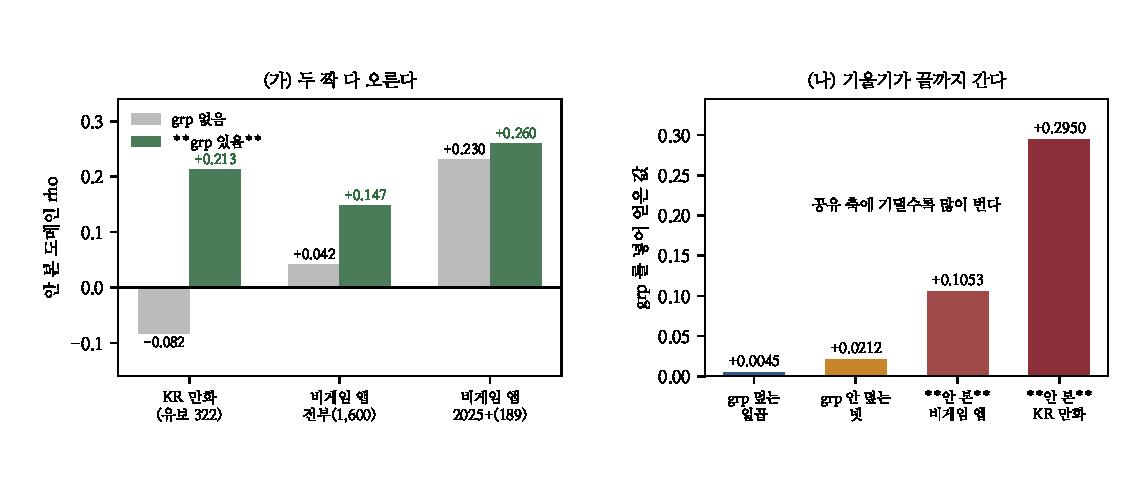
\includegraphics[width=\textwidth]{figs/fig418.pdf}
\caption{(가) 안 본 도메인 두 짝 모두 grp 로 오른다. (나) 노트 413에서
시작한 기울기의 네 눈금.}
\end{figure}

\end{document}
